% Preamble
% ---
\documentclass{article}

% Packages

% \usepackage{graphicx}
% \usepackage{subfig}

\usepackage{multicol}
\usepackage{float}

\usepackage{tikz}
\usepackage{pgfplots}
\usepgfplotslibrary{external}
% \usetikzlibrary{shapes.geometric, arrows}
% 
\usepackage[english]{babel}
\usepackage{hyperref} % 1 -> Figure 1
\usepackage{caption}

% code block
\usepackage{xcolor}
\usepackage{listings}

\definecolor{mGreen}{rgb}{0,0.6,0}
\definecolor{mGray}{rgb}{0.5,0.5,0.5}
\definecolor{mPurple}{rgb}{0.58,0,0.82}
\definecolor{backgroundColour}{rgb}{0.95,0.95,0.92}

\lstdefinestyle{CStyle}{
    backgroundcolor=\color{backgroundColour},   
    commentstyle=\color{mGreen},
    keywordstyle=\color{magenta},
    numberstyle=\tiny\color{mGray},
    stringstyle=\color{mPurple},
    basicstyle=\footnotesize,
    breakatwhitespace=false,         
    breaklines=true,                 
    captionpos=b,                    
    keepspaces=true,                 
    numbers=left,                    
    numbersep=2pt,                  
    showspaces=false,                
    showstringspaces=false,
    showtabs=false,                  
    tabsize=2,
    language=C
}

\pgfplotscreateplotcyclelist{mylist}{%
red,every mark/.append style={fill=red!80!black},mark=*,mark size=3pt\\%
brown!60!black,every mark/.append style={fill=brown!80!black},mark=*, mark size=3pt\\%
black,every mark/.append style={fill=black!80!black},mark=*, mark size = 3pt\\%
}


\usepackage{geometry}
\geometry{margin=1.2cm}

\title{Optimisation of d2q9-bgk Lattice Boltzmann Scheme}
\author{James Elgar, za18968}
\date{\today}

% ---

% \graphicspath{ {assets/} }

% \setlength{\columnsep}{1.3cm}

% \setlength{\columnsep}{0.8cm}
\begin{document}
\begin{multicols}{2}

\maketitle

\section{Introduction}

This report will explore the optimizations applied to the implementation of
a given algorithm to solve a d2q9-bgk Lattice Boltzmann scheme.  Starting with
an unoptimized serial implementation, it will apply three stages of optimisation
and compare the results. The first stage will be serial optimisations which
make the general algorithm more efficient mainly by reducing the number of
parses over the cells array to one, reducing the memory bandwidth required. The
second stage will make use of SIMD, single instruction multiple data, where the
compiler can vectorize certain sections of the algorithm allowing it to compute
multiple data values with single instructions by making use of vector registers
and instructions. The final stage will explore using OpenMP to run section of
the algorithm in parallel and convey the large benefits of being able to spread
out the required computation over multiple cores. However it will also look at
the limitation of this approach as memory bandwidth and sharing can continue to
limit performance. Throughout the stages few changes will be made to the
underlying implementation of the algorithm and the majority of the optimisation
will come from assisting the compiler and the OpenMP library with the
optimisations they are able to achieve.

\section{Serial Optimisation}

\subsection{Compiler options}

Many modern compilers provide various options to optimize the given code,
simply by adding compiler flag options. The "O" flags offer various levels of
optimisation with \verb|-O3| being the highest.

\autoref{tab:compilerflags} shows the run time of the serial optimized code
(without vectorization) with different compiler flags. This shows that by
simply using the \verb|-Ofast| flag, when compared to no optimisations
(\verb|-O0|), there can be a 4x decrease in run time. In later sections
additional compiler flags were added to optimize the other stages (such as
vectorization). The compiler flags used in the final implementation were 

\begin{itemize}
  \item \verb|-fast| - icc specific flag which includes -Ofast and a few other
    optimisations
  \item \verb|-mtune=native| and \verb|-xAVX| allow for the compiled binary to
    be specific to the current environment. \verb|xAVX| explicitly specific the 
    type of SIMD instructions to target (based on the architecture).
  \item \verb|-no-prec-sqrt| reduces the required precision of the square root
    function.
\end{itemize}

\begin{center}
 \begin{tabular}{ |p{5cm}||p{1.5cm}| }
 \hline
 \multicolumn{2}{|c|}{Results} \\
 \hline
 Compiler flag & Run time \\
 \hline
 -O0                  & 111.7   \\
 -O1                  & 34.5   \\
 -O2                  & 34.2   \\ 
 -O3                  & 31.9   \\ 
 -Ofast               & 26.8   \\ 
 -Ofast -mtune=native & 26.5   \\
 \hline
\end{tabular}
\captionof{table}{Serial run time with different compiler flags}
\label{tab:compilerflags}
\end{center}

\subsection{Reduce Memory Accesses}

In the original implementation of the algorithm, for each timestep the
\verb|cells| array was looped over 4 times, in \verb|propagate|,
\verb|rebound|, \verb|collision| and \verb|av_velocity|. This resulted in
repeated stores and loads of the same sections of memory. To prevent this the
first 3 separate functions (those in the \verb|timestep| function) were fuzed
into a single loop. This meant the same sections of memory were used closer
together making it is more likely for them to still be in cache. This therefore
reduces the memory bandwidth used and since this implementation is memory bound
results in a increase in performance. The function \verb|av_velocity| was also 
repeating calculations that already took place in collision and requiring an
additional loop over cells. The result was therefore calculated in the single
parse over the cells, reducing the need for this additional loop. 

Another issue with the original implementation was in  propagate and collisions
where the values were switched between \verb|tmp_cells| and \verb|cells| multiple
times which results in a waste of memory bandwidth as unnecessary loads and
stores take place. In the new implementation the \verb|tmp_cells| array was
used as the "answer" space and stores only the next timestep's cell values.
This then only required a single write to \verb|tmp_cells| each timestep. At
the end of the timestep the \verb|tmp_cells| and \verb|cells| array's pointers
were then swapped which set the \verb|cells| array to the correct value without
having to write directly to the array. Overall these optimisations reduced the 
runtime of the serial implementation from 38.5 seconds to 26.4.

\subsection{Vectorisation}

Having improved the implementation of the serial code, there is now a clear
critical section (the section which takes the most time), inside the single
pass of the cell's grid. This is where the majority of the computation takes places
and thus is where most of the time of the program is used. Since this section
preform repeat operations on the input array, there is an additional serial
approach to optimization.

Modern CPU architectures include vector registers and instructions. This allows
for computation to take place on a vector of values whilst only using a single
instruction. This approach is known as SIMD, (single-instruction multiple
data). When enabled, compilers are able to automatically make use of these
vector instructions. For this algorithm, this has the potential for large
performance gains as fewer instructions are required for the cells array in the
critical section.

\begin{lstlisting}[style=CStyle, label={lst:cellsdataalign}, caption={Example of memory allignment for a cells array.},]
  // Allocate aligned data
  cells_ptr->speed0 = _mm_malloc(params->nx * params->ny * sizeof(float), 64);
  // When using the array allow the compiler to assume alignment
  __assume_aligned(cells->speed0, 64);
\end{lstlisting}

In many cases the compiler is able to automatically vectorize code blocks.
However if the data is not aligned then the compiler will have to complete a prior
step, called the "prologue"\cite{vsaac} step, to process this unaligned data, or
alternatively use unaligned instructions (which are less efficient). The
compiler is also not able to assume that an array of floats, such as the arrays
of speeds in the new \verb|t_speed| struct are aligned. Therefore it will have
to complete this prior step regardless. To prevent this the arrays can be
aligned when they are created using the \verb|__mm_malloc| function, as shown in \autoref{lst:cellsdataalign}. This
ensure the created array is aligned on the request boundary, in this case 64
bytes was used to match the size of the cache line in an \emph{Intel Xeon
e5-2680}. Compiler directives can then be use to tell the compiler that the arrays
are aligned. This allows the compiler to skip the "proluge" step and use the
aligned instructions. This significantly reduces the overhead of vectorizing as
well as making it more likely for the compiler to automatically vectorize the
given section.

Another useful hint to assist the compiler in its optimizations is to use the
\verb|restrict| keyword. This tells the compiler to prevent pointer aliasing,
which ensures the target value will only be accessed through the restricted
pointer (not another aliased pointer). In practical terms this reduces the
number of times the pointer value has to be fetched from memory as the cached
value can be used repeatedly without the risk of it having changed as a result
of an overlap between pointer (in this case there would be a risk of overlap
with \verb|cells| and \verb|tmp_cells|). In a memory bound problem this can
therefore be an important step in reducing the memory bandwidth used.

\begin{lstlisting}[style=CStyle, label={lst:assumecellssize}, caption={Additional compiler hints},]
  __assume(params.nx%128==0);
  __assume(params.ny%128==0);
\end{lstlisting}

The intel compiler also allows for other hints to be provided. In this
implementation hints were added to inform the compiler about the size of the
cells array (and therefore the size of the loops). As show in the example in
\autoref{lst:assumecellssize}, the \verb|__assume| directive was used, to tell
compiler that the size of the cells array was divisible by various given powers of 2.
In the implementation all powers of 2, up to a maximum of 128 were provided (as
this was the maximum input size). This should further assist the compiler in
its optimizations, especially when vectorizing the inner loop.

The final step to ensuring the code was vectorized was to add the compiler
directive \verb|#pragma omp simd| to the inner for loop. This explicitly tells
the compiler that this section of the code should be vectorized. 

This alone, although successfully vectorizing the loop, did not result in a
significant performance gain. Observing the Roofline graph showed that this
version of the vectorized code was very heavily memory bandwidth bound. This
was as a result of the data layout of the cells array. 

In the original implementation the speeds for each cell were stored in a
structure (\verb|t_speed|) and the whole grid of cells was an array of these
structures. This implementation does not lend it self to vectorization as it
can result in unnecessary fetches from memory. This is because when a single
speed value is fetch an entire cache line (64 bits) will be used to fetch the
structure. This results in a waste of memory bandwidth as the rest of the
cache line is not used and only the single float value for that speed is actually
required. Therefore switching the implementation to use a structure of arrays
(where each speed is a separate array) allowed the code to be vectorized more
efficiently as each fetch for a speed only fetched a single float and therefore
reduced the overall memory bandwidth required. 

When comparing the Roofline results in \autoref{fig:rlserial} we can see a
large improvement in the performance, from 2.49 GLOPs to 13.2 GLOPs, once the
vectorization is introduced. These improvements are as a direct
result of vectorization and the update to the data layout which reduces the
memory bandwidth requirements. The Intel compiler also provides a vectorized
implementation for the \verb|sqrt| function which allows for the majority of
the computation in the critical section to be vectorized.

Despite the large improvements, it may have been expected to see a larger
improvement when the majority of instructions are now vectorized. In the
critical section this vectorization could be expected to reduce the number of
required instruction by a significant factor as a result of the vector length
being 32 bits. However such a large improvement is not observed as the problem
remains memory bandwidth bound meaning as the number of instructions is reduces
and the size of the vectors increase, the memory bandwidth required increases
as more data is required at to compute these vector instructions. Moreover
there is some additional overhead to vectorizing the code and thus this will
impact the overall run time.

Overall the use of vectorization reduces the run time by a factor of 2.7 to 3.5
times as shown in \autoref{tab:stageruntimes}. It is therefore a very valuable
approach in order to reduce the run time, however it can require some
significant changes to the algorithm in order to setup efficiently such as
ensuring the correct data layout and alignment.


\begin{tikzpicture}
\begin{axis}[
  xmode = log,
  ymode = log,
  axis lines = left,
  xlabel = Operational Intensity (FLOPS/byte),
  ylabel = Double precision GFLOPS/s (Scalar),
  ymin = 1e-2,
  xmin = 0.0029,
  ymax = 1000,
  xmax = 1,
  scaled ticks=true,
  legend pos=south east,
  cycle list name=mylist
]

% Original implementation 
% \addplot coordinates {
%   (0.457, 4.911)
% } node[left, ] (TextNode) {$(0.46, 4.91)$};
% \addlegendentry{Serial (Original Implementation)}

% Serial (No vectorizing)
\addplot coordinates {
  (0.341, 2.492)
} node[below left, ] (TextNode) {$(0.34, 2.49)$};
\addlegendentry{Serial (No vectorization)}

% Serial (No vectorizing)
\addplot coordinates {
  (0.383, 13.206)
} node[above left, ] (TextNode) {$(0.38, 13.2)$};
\addlegendentry{Serial (With vectorization)}

%DRAM
\addplot[color=blue] coordinates {
  (0.0029, 0.21)
  (0.77, 57.29)
  (100, 57.29)
} node[near start, above, sloped] (TextNode) {DRAM, 75GB/s};

%L1
\addplot[color=blue] coordinates {
  (0.0029, 25.07)
  (0.0065, 57.29)
  (100, 57.29)
} node[near start, above, sloped] (TextNode) {L1, 8830/s};

\end{axis}
\end{tikzpicture}
\captionof{figure}{Roofline analysis for serial implementations}
\label{fig:rlserial}

\begin{tikzpicture}
\begin{axis}[
  xmode = log,
  ymode = log,
  axis lines = left,
  xlabel = Operational Intensity (FLOPS/byte),
  ylabel = Double precision GFLOPS/s (Scalar),
  ymin = 0.5e-6,
  xmin = 0.5e-6,
  ymax = 10000,
  xmax = 100,
  scaled ticks=true,
  legend pos=south east,
  cycle list name=mylist
]

% Critical section
\addplot coordinates {
  (0.382, 119)
} node[below right, ] (TextNode) {$(0.382, 119)$};
\addlegendentry{28 cores parallel}

%DRAM
\addplot[color=blue] coordinates {
  (4.25e-7, 3.18e-5)
  (22.2, 1656)
  (100, 1656)
} node[midway, above, sloped] (TextNode) {DRAM, 75GB/s};
%
%L1
\addplot[color=blue] coordinates {
  (4.25e-7, 0.0032)
  (0.19, 1656)
  (100, 1656)
} node[midway, above, sloped] (TextNode) {L1, 8830GB/s};

\end{axis}
\end{tikzpicture}
\captionof{figure}{Roofline analysis for parallel implementations}
\label{fig:rlparallel}

\section{Parallel (OpenMP)}

Having optimized the inner loop in the above section the next optimization that
can be used is to run the loops in parallel. In this implementation the outer
loop was run in parallel while the inner loop maintained the other
optimizations. This parallelism was achieved by using the OpenMP
library. This library provides a collection of compiler directives which can be
used to write parallel shared memory programs.

The first step in order to run the loop in parallel is to turn on OpenMP for the
compiler with the \verb|-qopenmp| flag. With this the OpenMP library is available to use.
At a basic level adding the \verb|parallel| and \verb|for| constructs should
allow the loop to run in parallel. The \verb|parallel| directive tells the
compiler to run the preceding block in parallel and \verb|for| tells it to
distribute the work of the following for loop evenly across the threads.

It is then important to handle the memory sharing that takes place in the loop.
Since the \verb|av_velocity| is also calculated in this loop each loop is
required to calculate the total number of cells without obstacles and the sum
of the magnitude of the velocity for these cells. When running the code with
just the \verb|#pragma omp parallel for| directive, the wrong answer is
obtained. This is because the values required to calculate \verb|av_velocity|
are in shared memory and thus every thread is competing to set the shared
values rather than accumulating the values across all the threads.

In order to efficiently calculate these shared sums a \verb|reduction| is
required. The \verb|reduction| directive tells the compiler that the given
variable is going to be accumulated over the duration of the parallel region. This allows
each thread to calculate its own sum without having to synchronize the global
shared value on every write. Once the forked section is complete and the
threads synchronize then all the sums can be combined to determine the final
value of the accumulated variables. This is significantly faster than requiring a
synchronized section during the fork as the threads can run independently and not have to wait
for each thread to synchronize the sum or lock and unlock (in the case of an
atomic variable) the values.

Another consideration when writing a parallel program is the number of cores
to use. In a bluecrystal node there are 2 sockets, which house 2 \emph{Intel
Xeon e5-2680} CPUs. Each of these CPUs have 14 cores, giving a total of 28
cores per node. \autoref{tab:parallelresults} and \autoref{fig:parallelresults}
show the run times of the parallel code on different numbers of cores. In the
larger problems (1024x1024) it is clear that as the number of cores increases
the run time decreases. Initially, between 1 and 4 cores, the rate of decrease
is linear, meaning as the number of cores increases the run time is halved.
This is as a result of the work in the critical section being shared over a
larger pool of cores and thus the total time of the forked region is decreased.

However this linear relationship becomes a sub-linear plateaus as the number of
cores increases. The reason for this can be observed in
\autoref{fig:rlparallel} which shows the Roofline analysis for the parallel
algorithm running on 28 cores. The results lie in the memory bound region,
this is as a result of the memory bandwidth becoming saturated as the number of
cores are increased and thus the computation rate increases at a faster rate
than the memory bandwidth available. 

However in the smaller problems there is a reduction in run time after 14
cores. This is observed as once the core count is above 14, two sockets are in
use (both CPUs) and therefore memory sharing between the sockets is required.
This is where a shared section of memory is in the cache of the other
socket so in order to access that section of memory a request has to be routed
through the other socket. This takes approximately two times as long as
fetching from the socket's local cache. For this reason when running the
algorithm on smaller grid sizes (such as 128x128) only 14 cores were used. This
removes this problem completely as only a single socket is used so all cache
accesses are for the local CPU's cache.

In general this non-uniform memory access, NUMA, can be mitigated by pinning 
the threads to a specific core. Setting \verb|OMP_PROC_BIND| to \verb|close|
tells OpenMP to bind the threads to specific cores and also as the threads are
assigned, ensure they are assigned to the threads closest to the master (main)
thread. Assigning \verb|OMP_PLACES| to \verb|cores| ensures that each
core is used as a single place (and no core sharing occurs such as
hyper-threading). Although the threads are now pinned to individual cores this
does not mean that the NUMA problem is reduced. This is because during the
memory assignment, in the \verb|initialise| function, the initial values for the
cells array are assigned serially (on a single thread). This means all the
values will in exist the same cache, linked to this single NUMA region. This
can be prevented by ensuring the initialisation of the values is parallelized
in the same way as the it is accessed in the critical region. In this case this
means also using the \verb|#pragma omp parallel for| directive when assigning the initial
values to the cells array. This will ensure the data is allocated in the same
NUMA region to which it is going to be required in the critical loop. The
combination of these factors should therefore reduce the number of
socket-to-socket memory requests allowing for the average time for each memory
access to be reduced.  

When comparing the run times of the parallel code with the vectorized
implementation in \autoref{tab:stageruntimes}, for larger problem sizes we see
an almost 14x reduction. Similarly when comparing the Roofline analysis in
\autoref{fig:rlserial} and \autoref{fig:rlparallel} an over 9 times improvement
in performance is observed. However similarly to the vectorized code we do not
observe a 28 times improvement as may be expected when running over 28 cores.
This is as a result of the memory saturation and the overhead of forking and
then synchronising the code. In smaller problems this overhead and the need for
memory sharing can even result in reduced performance as the core count increases
after a certain point.

% \begin{lstlisting}[style=CStyle, label={lst:ompparallelloop}, caption={TODO},]
% #pragma omp parallel for schedule(static) reduction(+:tot_cells) reduction(+:tot_u)
%     for (int jj = 0; jj < params.ny; jj++)
%     {    
% #pragma omp simd aligned(cells:64) aligned(tmp_cells:64) aligned(obstacles:64) reduction(+:tot_cells) reduction(+:tot_u)
%       for (int ii = 0; ii < params.nx; ii++)
%       {
%         ...
%       }
%     }
% \end{lstlisting}

% \begin{tikzpicture}
% \begin{axis}[
%   axis lines = left,
%   xlabel = Number of cores,
%   ylabel = Run time (seconds),
%   xmin = 0,
%   ymin = 1,
% ]
% % 1028x1028
% \addplot[color=red] table {
%   1   11.17
%   2   10.48
%   4   14.45
%   6   53
%   8   43 
%   10  42
%   12  39.5
%   14  39.1
%   16  37.1
%   18  32.6
%   20  26.6
%   22  26.3
%   24  22.8
%   26  21.0
%   28  85.91
% };
% \end{axis}
% \end{tikzpicture}

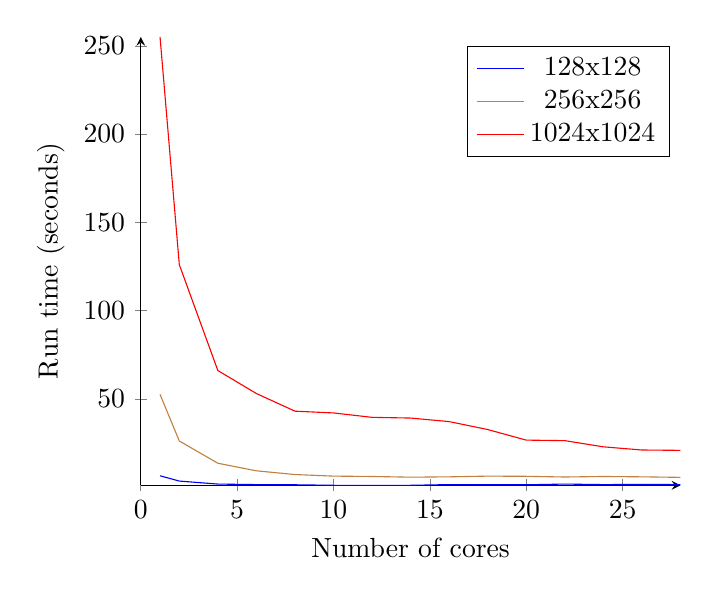
\begin{tikzpicture}
\begin{axis}[
  axis lines = left,
  xlabel = Number of cores,
  ylabel = Run time (seconds),
  xmin = 0,
  ymin = 1,
]
% 128x128
\addplot[color=blue] table {
  1   6.4
  2   3.4
  4   1.7
  6   1.4
  8   1.3
  10  1.0
  12  0.9
  14  1.0
  16  1.4
  18  1.3
  20  1.3
  22  1.7
  24  1.4
  26  1.5
  28  1.4
};
\addlegendentry{128x128}

% 256x256 
\addplot[color=brown] table {
  1   52.5
  2   26.1
  4   13.5
  6   9.2
  8   7.1
  10  6.2
  12  6.0
  14  5.6
  16  5.8
  18  6.2
  20  6.1
  22  5.7
  24  6.0
  26  5.8
  28  5.5
};
\addlegendentry{256x256}

% 1028x1028
\addplot[color=red] table {
  1   255
  2   126
  4   66
  6   53
  8   43 
  10  42
  12  39.5
  14  39.1
  16  37.1
  18  32.6
  20  26.6
  22  26.3
  24  22.8
  26  21.0
  28  20.8
};
\addlegendentry{1024x1024}
\end{axis}
\end{tikzpicture}
\captionof{figure}{Parallel scaling results for 1-28 cores on 3 grid sizes}
\label{fig:parallelresults}

\begin{center}
  \begin{tabular}{ |p{1.5cm}||p{1.5cm}|p{1.5cm}|p{1.5cm}| }
 \hline
 \multicolumn{4}{|c|}{Results} \\
 \hline
 Number of cores & 128x128 & 256x256 & 1024x1024 \\
 \hline
 1  & 6.4 &  52.5  &  255.4   \\
 2  & 3.4 &  26.1  &  126.2   \\
 4  & 1.7 &  13.5  &  66.1    \\ 
 6  & 1.4 &  9.2   &  53.3    \\ 
 8  & 1.3 &  7.1   &  43.4    \\ 
 10 & 1.0 &  6.2   &  42.4    \\
 12 & 0.9 &  6.0   &  39.7    \\
 14 & 1.0 &  5.6   &  39.1    \\ 
 16 & 1.4 &  5.8   &  37.1    \\ 
 18 & 1.3 &  6.2   &  32.6    \\
 20 & 1.3 &  6.1   &  26.6    \\
 22 & 1.7 &  5.7   &  26.3    \\ 
 24 & 1.4 &  6.0   &  22.8    \\ 
 26 & 1.5 &  5.8   &  21.0    \\ 
 28 & 1.4 &  5.5   &  20.8    \\
 \hline
\end{tabular}
\captionof{table}{Parallel scaling results for 1-28 cores}
\label{tab:parallelresults}
\end{center}

\begin{center}
  \begin{tabular}{ |p{1.5cm}||p{1cm}|p{1.5cm}|p{2cm}| }
 \hline
 \multicolumn{4}{|c|}{Results} \\
 \hline
 Grid size & Serial & Vectorised & Parallel(cores) \\
 \hline
 128x128    & 26.4  & 7.4   &  1.15(14)   \\
 128x256    & 53.3  & 16.1  &  1.85(14)   \\
 256x256    & 213.6 & 59.6  &  5.68(28)   \\
 1024x1024  & 869.1 & 318.9 &  20.8(28)    \\ 
 \hline
\end{tabular}
\captionof{table}{Run times for optimisation stages}
\label{tab:stageruntimes}
\end{center}

\section{Conclusion}

Modern compilers offer many powerful options to assist in code optimisation.
Often the most efficient approach to optimising a code can be to assist the
compiler in its own optimisations. Simple changes such as using compiler
optimisation flags can have a profound impact on the runtime of the algorithm.
Similarly with the correct hints and memory aligned compilers are able to
automatically vectorize a given code. This can dramatically reduce the run time
by allowing a vector instructions to compute multiple values and thus reduce the
overall number of instructions required. In this implementation, the vectorized code ran
over 2.5 times faster than the optimised serial version with an approximately 5
times increase in performance. Once a code is well optimised in serial further
improvements can be gained by making sections of the program run in parallel.
This can dramatically increase the performance of the code as the work is
shared across multiple cores. With modern processors often having high core
counts, this can also result in large performance gains.  Similarly to
vectorization, using OpenMP directives and environment variables, parallelized
code can be achieved with little changed to the implementation. In this running
the critical sections in parallel resulted in up to a 13 times reduction in
overall run time on the largest problem size.


\bibliographystyle{unsrt}
\bibliography{report}

\end{multicols}
\end{document}
